\documentclass[slovene,11pt,a4paper]{article}
\usepackage[margin=2cm,bottom=3cm,foot=1.5cm]{geometry}
\setlength{\parindent}{0pt}
\setlength{\parskip}{0.5ex}

\usepackage[pdftex]{graphicx}
\DeclareGraphicsExtensions{.pdf,.png}


\usepackage{amsmath}
\usepackage{amsfonts}
\usepackage{mathrsfs}
\usepackage[usenames]{color}
\usepackage[slovene]{babel}
\usepackage[utf8]{inputenc}
\usepackage{siunitx}
\usepackage{hyperref}


% \def\phi{\varphi}
\def\eps{\varepsilon}
\def\theta{\vartheta}

\newcommand{\thisyear}{2025/26}

\renewcommand{\Re}{\mathop{\rm Re}\nolimits}
\renewcommand{\Im}{\mathop{\rm Im}\nolimits}
\newcommand{\Tr}{\mathop{\rm Tr}\nolimits}
\newcommand{\diag}{\mathop{\rm diag}\nolimits}
\newcommand{\dd}{\,\mathrm{d}}
\newcommand{\ddd}{\mathrm{d}}
\newcommand{\ii}{\mathrm{i}}
\newcommand{\lag}{\mathcal{L}\!}
\newcommand{\ham}{\mathcal{H}\!}
\newcommand{\four}[1]{\mathcal{F}\!\left(#1\right)}
\newcommand{\bigO}[1]{\mathcal{O}\!\left(#1\right)}
\newcommand{\sh}{\mathop{\rm sinh}\nolimits}
\newcommand{\ch}{\mathop{\rm cosh}\nolimits}
\renewcommand{\th}{\mathop{\rm tanh}\nolimits}
\newcommand{\erf}{\mathop{\rm erf}\nolimits}
\newcommand{\erfc}{\mathop{\rm erfc}\nolimits}
\newcommand{\sinc}{\mathop{\rm sinc}\nolimits}
\newcommand{\rect}{\mathop{\rm rect}\nolimits}
\newcommand{\ee}[1]{\cdot 10^{#1}}
\newcommand{\inv}[1]{\left(#1\right)^{-1}}
\newcommand{\invf}[1]{\frac{1}{#1}}
\newcommand{\sqr}[1]{\left(#1\right)^2}
\newcommand{\half}{\frac{1}{2}}
\newcommand{\thalf}{\tfrac{1}{2}}
\newcommand{\pd}{\partial}
\newcommand{\Dd}[3][{}]{\frac{\ddd^{#1} #2}{\ddd #3^{#1}}}
\newcommand{\Pd}[3][{}]{\frac{\pd^{#1} #2}{\pd #3^{#1}}}
\newcommand{\avg}[1]{\left\langle#1\right\rangle}
\newcommand{\norm}[1]{\left\Vert #1 \right\Vert}
\newcommand{\braket}[2]{\left\langle #1 \vert#2 \right\rangle}
\newcommand{\obraket}[3]{\left\langle #1 \vert #2 \vert #3 \right \rangle}
\newcommand{\hex}[1]{\texttt{0x#1}}

\renewcommand{\iint}{\mathop{\int\mkern-13mu\int}}
\renewcommand{\iiint}{\mathop{\int\mkern-13mu\int\mkern-13mu\int}}
\newcommand{\oiint}{\mathop{{\int\mkern-15mu\int}\mkern-21mu\raisebox{0.3ex}{$\bigcirc$}}}

\newcommand{\wunderbrace}[2]{\vphantom{#1}\smash{\underbrace{#1}_{#2}}}

\renewcommand{\vec}[1]{\overset{\smash{\hbox{\raise -0.42ex\hbox{$\scriptscriptstyle\rightharpoonup$}}}}{#1}}
\newcommand{\bec}[1]{\mathbf{#1}}

\title{
\sc\large Matematično-fizikalni praktikum \thisyear\\
\bigskip
\bf\Large 5.~naloga: Hitra Fourierova transformacija in korelacijske funkcije
}
\author{Samo Krejan, 28231092}
\date{}

\begin{document}
\maketitle
% \vspace{-1cm}

Diskretno Fourierovo transformacijo smo definirali kot
\begin{equation*}
H_k = \sum_{n=0}^{N-1}
h_n \exp(2 \pi \ii k n / N),
\qquad k=-\tfrac{N}{2},\dots ,\tfrac{N}{2},
\end{equation*}
oziroma
\begin{equation*}
H_k = \sum_{n=0}^{N-1} W_N^{nk} h_n,
\qquad W_N = \exp(2 \pi \ii / N).
\end{equation*}
Ta postopek ima očitno časovno zahtevnost $N^2$. Račun pa je
mogoče izvesti tudi z bistveno manj operacijami. Osnovni premislek
je razcep
\begin{equation*}
H_k = H_{k}^\mathrm{sod} + W_N^k H_{k}^\mathrm{lih} \>,  
\end{equation*}
kjer smo transformiranko $H$ izrazili s transformacijama njenih
sodih in lihih členov, pri čemer je vsota vsake od transformacij zdaj dolžine N/2.
 Gornjo relacijo lahko uporabljamo rekurzivno:
če je $N$ enak potenci števila 2, lahko rekurzijo razdrobimo
do nizov, ki imajo samo še en člen. Zanj je transformacija
identiteta. Za obrat pri eni vrednosti frekvence (pri danem $m$)
je potrebno na vsakem koraku rekurzije le eno množenje s potenco
$W$, korakov pa je $\log_2 N$.  Skupna časovna zahtevnost je torej
le še $N\log_2 N$.

Da ne iščemo pripadnikov niza po vsej tabeli, si podatke
preuredimo. Lahko je pokazati, da je v prvotni tabeli treba med
seboj zamenjati podatke, katerih vrstna števila v binarnem zapisu
so obrnjena: v novem redu jemljemo člene kar po vrsti. Tudi
potenc $W$ ne izražamo vedno znova s sinusi in kosinusi,
pač pa jih računamo z rekurzijo.  Tak ali podoben postopek
je osnova vseh algoritmov hitre Fourierove transformacije (FFT).

Z neko transformacijo iz družine FFT bomo izračunali korelacijsko
funkcijo dveh signalov. Korelacija periodičnih funk\-cij $g(t)$ in $h(t)$
s periodo $T$ je definirana kot:
\begin{equation*}
\phi_{gh}(\tau)=\frac{1}{T}\int\limits_0^{T} g(t+\tau)\,h(t)\dd t \>,  
\end{equation*}
oziroma diskretno
\begin{equation*}
  \phi_{gh}(n)= \frac{1}{N}\sum_{k=0}^{N-1} g_{k+n}\, h_k \>.
\end{equation*}
Računamo torej skalarni produkt funkcij, ki sta časovno premaknjeni
za $\tau$ oziroma $n$. Če je za določeno vrednost premika ta
funkcija višja kot v okolici, potem to pomeni, da sta si funkciji
podobni, le da ju je treba premakniti, da se to vidi.

V primeru, da sta funkciji (signala), ki ju primerjamo, enaki,
računamo njuno {\sl avtokorelacijsko funkcijo\/}: ta je mera
za to, ali signal ostaja s pretekanjem časa sam sebi podoben.
Če je signal slabo koreliran (sam s sabo), korelacija $\phi_{hh}(n)$
relaksira h kvadratu povprečnega signala $\langle h\rangle^2$, kjer je
\begin{equation*}
\langle h\rangle = \frac{1}{N} \sum_{k=0}^{N-1} h_k \>.  
\end{equation*}
Iz lokalnih maksimov v avtokorelacijski funkciji sklepamo
na periodičnosti, bodisi popolne ali približne.
Pri periodičnih signalih je tudi avtokorelacijska funkcija
striktno periodična, za stohastične procese pa je značilna
eksponentna avtokorelacijska funkcija.
še bolj nas zanima, kako {\sl hitro\/} se korelacija izgublja:
računamo rajši reskalirano obliko avtokorelacije
\begin{equation*}
\widetilde{\phi}_{hh}(n) = 
{ \phi_{hh}(n) - \langle h\rangle^2 \over \phi_{hh}(0) - \langle h\rangle^2 } \>,  
\end{equation*}
kjer je imenovalec nekakšno merilo za  varianco signala,
\begin{equation*}
\sigma^2 = \phi_{hh}(0) - \langle h\rangle^2 
= \frac{1}{N} \sum_{k=0}^{N-1} \left( h_k - \langle h\rangle \right)^2 \>.  
\end{equation*}
Pri zgornjih enačbah moramo še ``peš'' poskrbeti za periodično
zaključenost signala pri $n=N$, torej da je perioda enaka velikosti
vzorca.  Če tega ne moremo narediti, je bolj pravilna definicija
avtokorelacije
\begin{equation*}
\phi_{hh}(n)= \frac{1}{N-n}\sum_{k=0}^{N-n-1} h_{k+n}\, h_k \>.  
\end{equation*}
Praktičen račun po zgornji formuli lahko postane za velike
vzorce prezamuden.  Avtokorelacijo rajši računamo s FFT (DFT) $\mathcal{F}$,
saj je korelacija obratna Fourierova transformacija ${\cal F}^{-1}$
produkta Fourierovih transformacij ${\cal F}$, torej z $G={\cal F}g$ in $H={\cal F}h$ dobimo
\begin{equation*}
\phi_{gh}(n) = \frac{1}{N-n}\mathcal{F}^{-1} \left[ G \cdot (H)^\ast \right]
\end{equation*}
oziroma
\begin{equation*}
  \phi_{hh}(n) = \frac{1}{N-n}{\cal F}^{-1} \left[ \, | H |^2 \, \right] \>.
\end{equation*}
Za račun s FTT signale dolžine $N$ najprej prepišemo v dvakrat
daljše, periodično zaključene podatkovne nize, $\widetilde{h}_n = h_n$,
$\widetilde{h}_{n+N} = 0$ za $n = 0, \ldots, N-1$
in $\widetilde{h}_{n+2N} = \widetilde{h}_{n}$.
Tedaj se avtokorelacija zapiše v obliki
\begin{equation*}
\phi_{hh}(n)={1\over N-n}\sum_{k=0}^{2N-1}\widetilde{h}_{k+n}\,\widetilde{h}_k \>,  
\end{equation*}
kar lahko izračunamo s FFT.

\section{Naloga}

Na spletni strani MF praktikuma najdeš posnetke
oglašanja velike uharice, naše največje sove.  Posneti sta
dve sovi z minimalnim ozadjem ({\tt bubomono} in {\tt bubo2mono})
in nekaj mešanih signalov, ki zakrivajo njuno oglašanje
({\tt mix}, {\tt mix1}, {\tt mix2} in {\tt mix22}).
V signalih {\tt mix2} in {\tt mix22} je oglašanje sove
komaj še zaznavno.  Izračunaj avtokorelacijsko funkcijo 
vseh signalov in poskusi ugotoviti, za katero sovo gre
pri teh najbolj zašumljenih signalih!

Poglejte si rutine {\tt four1\/} iz Numerical Recipes
ali knjižnice {\tt fftw3}, ki je še dosti hitrejša. V okolju Python
so te rutine vključene v 'fft' paket. 
(Pri tako velikih vzorcih je skorajda nujno uporabiti FFT
namesto počasne navadne DFT.)

\subsection{FFT}

Nalogo sem začel tako, da sem najprej naredil lastno implementacijo hitre Fourierove transformacijev Rust-u. Ta mi sicer ni uspela najbolje saj je med drugim delovala zgolj za sezname katerih dolžina je potenca števila 2 in pa, čeprav je dosegala natančnosti v bližini numerične zmogljivosti dvojne natančnosti, je bila mnogo počasnejša od $numpy.fft.fft$ implementacije (slika \ref{speed}), tako da sem se v nadaljevanju naloge odločil uporabljati kar $numpy$ implementacijo.

\begin{figure}[ht]
\begin{center}
    \includegraphics[width=10cm]{graphs/speed.pdf}
    \caption{Čas potreben za izvedbo FFT v odvisnosti od velikosti seznama (potence števila 2). Kvalitativno lahko vidimo, da časovna zahtevnost res ustreza $O(n\log n)$ in pa tudi, da je numpy implementacija mnogo boljša.}
    \label{speed}
\end{center}
\end{figure}

\subsection{Avtokorelacijska funkcija}

Ker bomo kasneje naredili avtokorelacijo signalov z hitrim vzorčenjem je pomembno, da poskrbimo, da je algoritem s katerim računamo avtokorelacijo čim bolj učinkovit. Zato sem analiziral tri implementacije avtokorelacije, sicer:

1. Osnovna implementacija v Pythonu po definiciji iz uvoda:
\begin{equation*}
\phi_{hh}(n)= \frac{1}{N-n}\sum_{k=0}^{N-n-1} h_{k+n}\, h_k \>.  
\end{equation*}

2. Po definiciji iz uvoda z "zero padding" za uporabo $numpy$:
\begin{equation*}
\phi_{hh}(n)={1\over N-n}\sum_{k=0}^{2N-1}\widetilde{h}_{k+n}\,\widetilde{h}_k \>,  
\end{equation*}

3. Navsezadnje pa še z uporabo FFT algoritma, kot je opisano v uvodu:
\begin{equation*}
  \phi_{hh}(n) = \frac{1}{N-n}{\cal F}^{-1} \left[ \, | H |^2 \, \right] \>.
\end{equation*}

Uspešnost avtokorelacije zašumljenega signala harmonikov in potrebnim časom za vsako iteracijo, sem prikazal na grafu \ref{test}

\begin{figure}[ht]
\begin{center}
    \includegraphics[width=12cm]{graphs/testni.pdf}
    \caption{Signal, njegova avtokorelacija (bralec naj bo pozoren na zamike za namen lepšega prikaza), ter časovna zahtevnost}
    \label{test}
\end{center}
\end{figure}

Takoj opazimo, da je implementacija z FFT daleč najhitrejša, zato sem od te točke naprej uporabljal kar to. Poleg tega opazimo tudi, da je avtokorelirana funkcija izgubila precej šuma, kar je odlična posledica avtokorelacije, ki nam bo kasneje prišla prav.

\subsection{Analiza posnetkov}

Na tej točki sem končno opremljen z vsemi potrebnimi orodji, da se lotim analize posnetkov sov. Najprej sem uporabil najbolj primitivno izmed orodij - lastna ušesa in iz poslušanja sklepal, da posnetek mix22 pripada sovi bubo2, medtem ko se mi zdi, da ostali pripadajo sovi bubo.

Predno pa sem se lotil potrjevati zgornjo hipotezo, sem želel dobiti še nekaj več občutka za posamezne posnetke, tako da sem z $matplotlib$ funkcijo $specgram$ najprej narisal spektogram posameznih posnetkov. Na ta način sem dobil grafe na sliki \ref{gram}

Sovi bo verjetno najlažje ločiti na podlagi frekvence skovikov, zato sem na prvi točki naredil zgolj Fourierovo transformacijo in dobil graf \ref{fft}

Hitro vidimo nekaj ujemanja med vrhovi frekvenc, a si sam, zaradi očitno mnogo šuma ne upam trditi, da dobljeni rezultati potrdijo mojo hipotezo. Zato sem se odločil narediti še relativno avtokorelacijsko funkcijo vseh posnetkov. Na ta način sem dobil graf \ref{ac}

Z dobljenimi grafi si nisem znal pomagati, nato pa sem se spomnil, kako avtokorelacija "polepša"\ podatke in bo tako Fourierova transformacija na avtokorelacijski funkciji izgledala bolje. Tako sem se odločil izvesti najprej avtokorelacijo in nato FFT in pa tudi dvakrat avtokorelacijo in nato FFT. Na ta način sem dobil sliki \ref{acfft} in \ref{acacfft}

Predvsem na zadnji sliki sedaj res lepo vidimo, da imata signala frekvenco pri precej distinktnih frekvencah (različni frekvenci skovika), tako da lahko končno z odločnostjo trdim, da imam očitno dovolj dober posluh, da lahko ločim dve sovi. Avtokorelacija in pa FFT sta se seveda pri tem izkazala kot dva ključna algoritma, ki misim, da sem jih uporabil uspešno.
\newpage

\begin{figure}[ht]
\begin{center}
    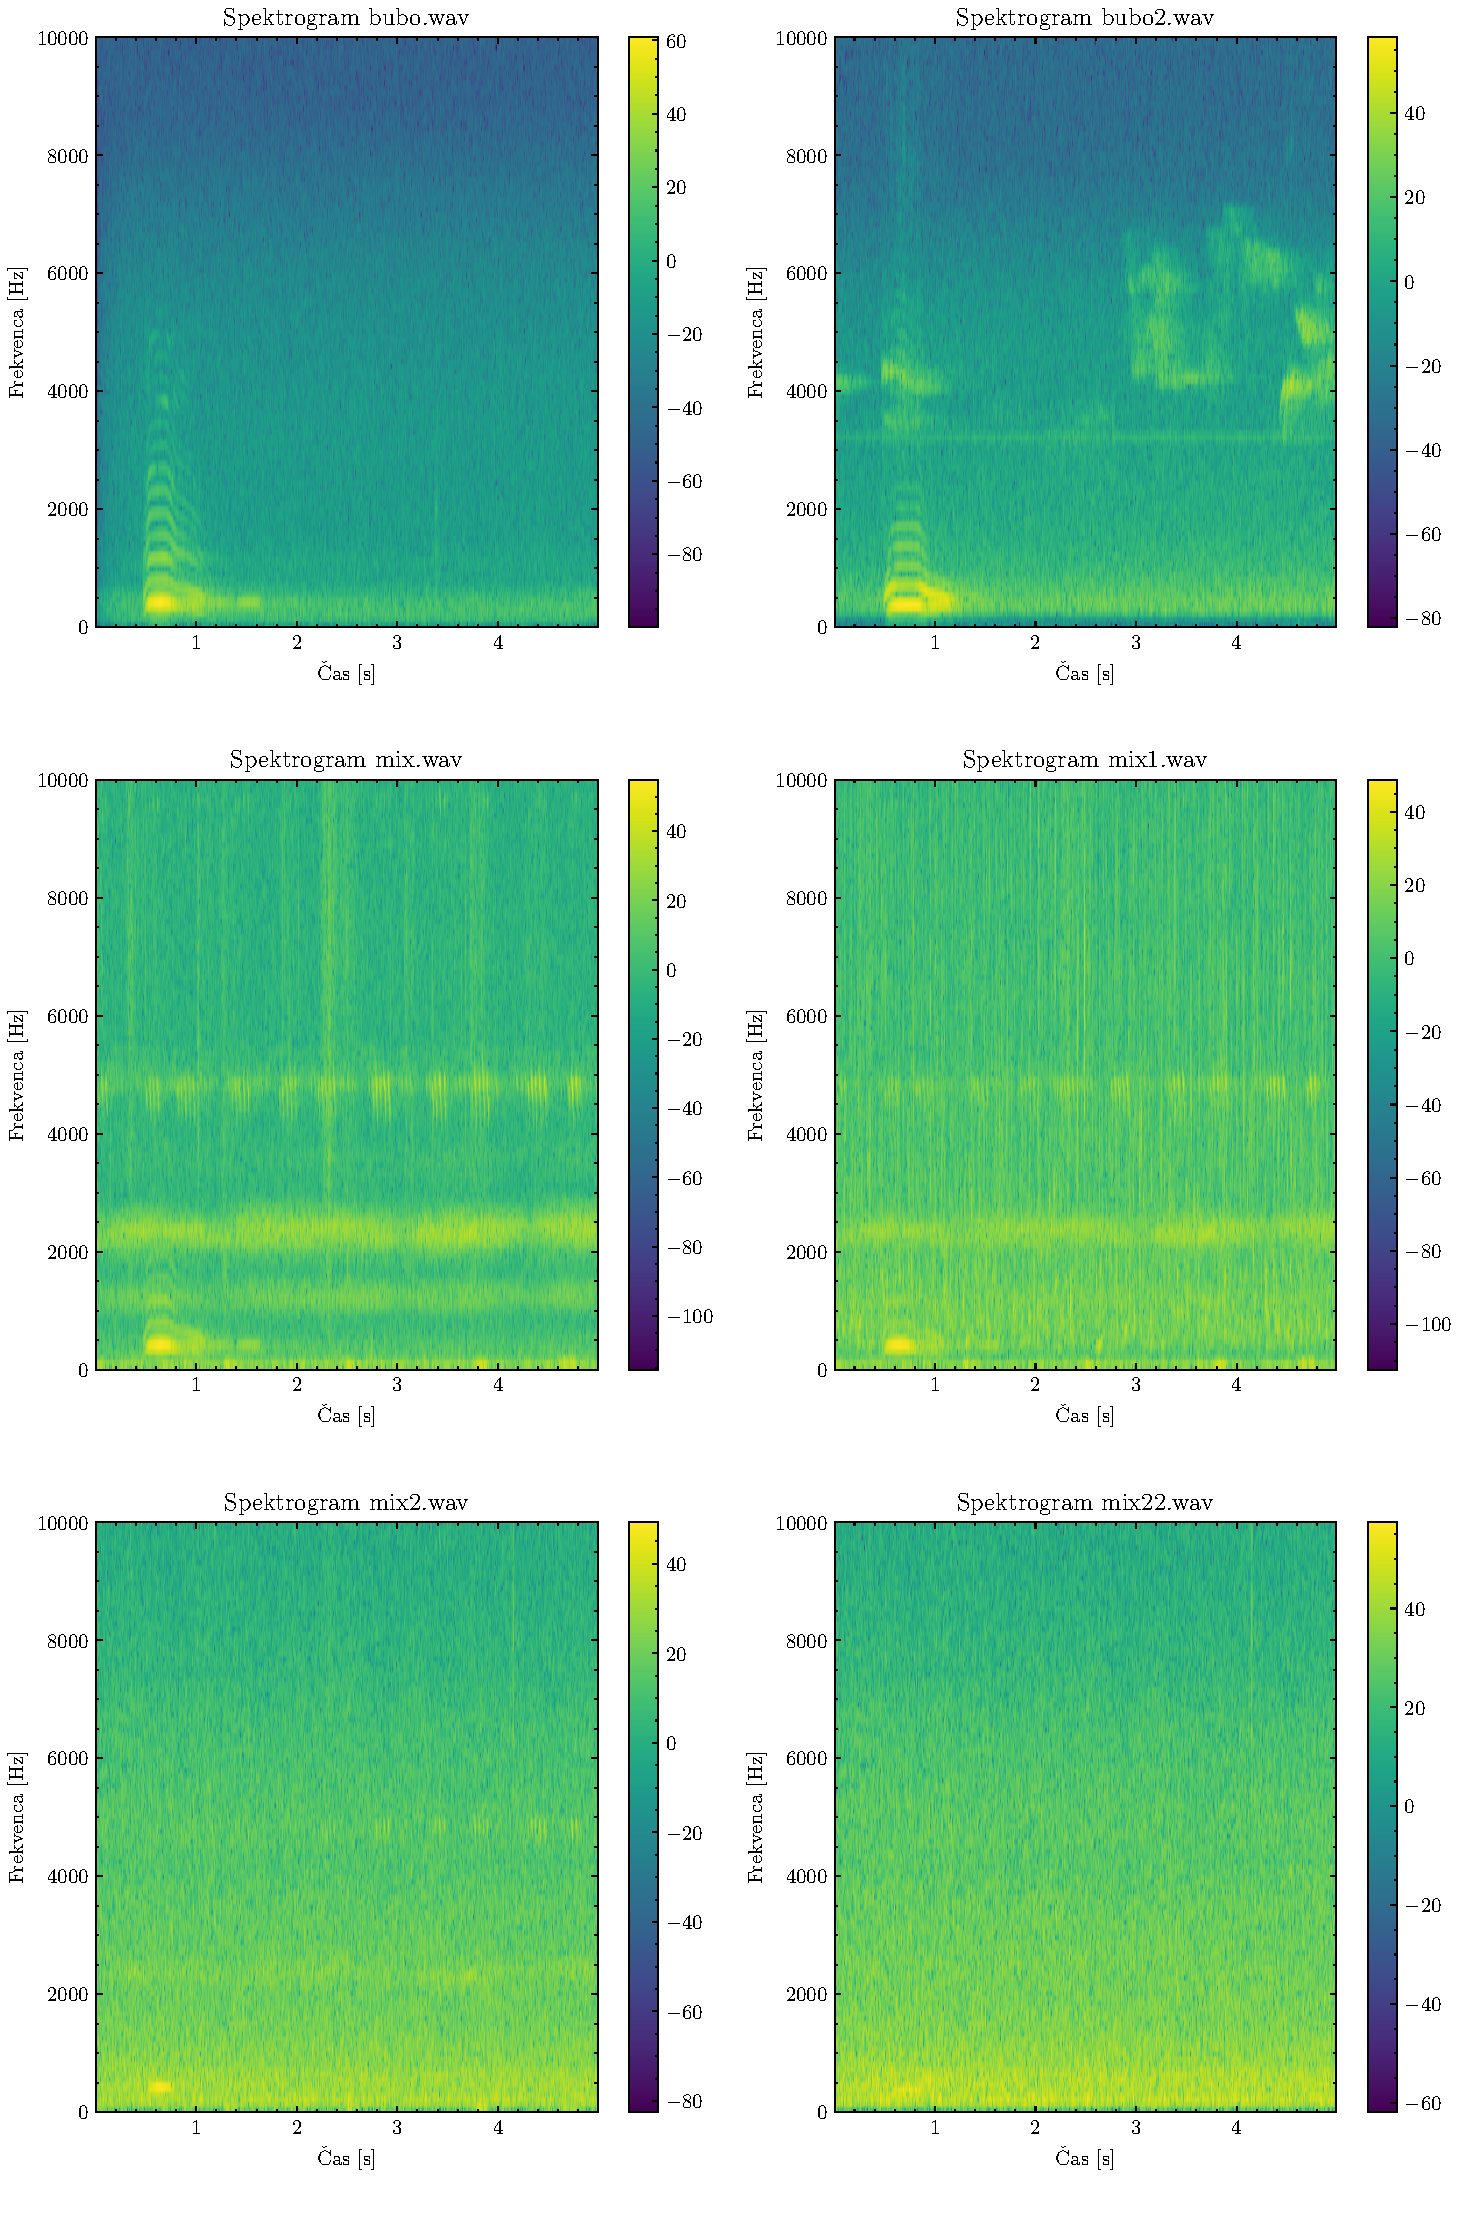
\includegraphics[width=14cm]{graphs/specgram.pdf}
    \caption{Spektogrami posnetkov. Nekatere lastnosti posnetkov lahko razberemo že iz spektrograma. Vidimo lahko naprimer, kako močno sta zašumljena posnetka mix2 in mix22, saj se na njima sam skovik vidi le še z nekaj domišljije. Poleg tega lahko na spektrogramu posnetka bubo vidimo celo višje frekvence skovika}
    \label{gram}
\end{center}
\end{figure}

\newpage

\begin{figure}[ht]
\begin{center}
    \includegraphics[width=13cm]{graphs/fft.pdf}
    \caption{Fourierova transformacija vseh posnetkov}
    \label{fft}
\end{center}
\end{figure}



\begin{figure}[ht]
\begin{center}
    \includegraphics[width=13cm]{graphs/ac.pdf}
    \caption{Avtokorelacijska funkcija vseh posnetkov}
    \label{ac}
\end{center}
\end{figure}


\newpage
\begin{figure}[ht]
\begin{center}
    \includegraphics[width=13cm]{graphs/acfft.pdf}
    \caption{Avtokorelacijska funkcija Fourierovo transformirana}
    \label{acfft}
\end{center}
\end{figure}

\begin{figure}[ht]
\begin{center}
    \includegraphics[width=13cm]{graphs/acacfft.pdf}
    \caption{Avtokorelacijska funkcija avtokorelacijske funkcije Fourierovo transformirana}
    \label{acacfft}
\end{center}
\end{figure}

\newpage

\section{Dodatna naloga}

Za dodatno nalogo sem se odločil na hitro analizirati uspešnost generatorjev naključnih števil. Primerjal sem numpy-jev random.random algoritem, in pa starodaven RANDU algoritem, ki ga je v 60ih razvil IBM. 

Naloge sem se lotil tako, da sem generiral seznamu naključnih števil dolžine $2^{25}$ najprej z enim in nato še z drugim algoritmom, in nato izvedel avtokorelacijsko funkcijo na posameznem seznamu. Idealen generator naključnih števil bi imel pri zelo dolgem seznamu avtokorelacijsko funkcijo povsod enako nič, razen pri zamiku nič. Kaj sem dobil dejansko za omenjena primera je razvidno na slikah \ref{nump} in \ref{rand}.

\begin{figure}[ht]
\begin{center}
    \includegraphics[width=10cm]{graphs/nump.pdf}
    \caption{Avtokorelacijska funkcija numpy-evega naključnega generatorja}
    \label{nump}
\end{center}
\end{figure}


\begin{figure}[ht]
\begin{center}
    \includegraphics[width=10cm]{graphs/rand.pdf}
    \caption{Avtokorelacijska funkcija RANDU naključnega generatorja}
    \label{rand}
\end{center}
\end{figure}


Kot vidimo je numpy-jev generator precej bolj uspešen, saj pri RANDU opazimo nekaj koreliranosti. Kljub temu mislim, da je glede na starost generatorja tudi RANDU precej uspešen.


\section{Zaključek}

Vaja je bila gotovo uspešeno izvedena, saj smo dosegli cilj in uspeli identificirati sove, tudi ko je bilo v ozadju mnogo ostalih zvokov. To nam je uspelo s pomočjo avtokorelacije in FFT algoritma, ki se izkažeta, kot dva izmed bolj pomembnih algoritmov, ko prido do iskanja vzorcev v signalih. 

Kljub eleganci algoritmov, mi je bila ta vaja najmanj všeč med vsemi do sedanjimi, verjetno tudi zato, ker sem imel zanjo najmanj časa in sem se tako težje poglobil v nalogo. Upam, da se to ne odraža nikjer drugje kot v uri oddaje naloge.

Sigurno se pomankanje časa odraža v poročilu pri poziciji grafov, ki so po dobri uri srdite borbe ostali nepremagani in samozavestno na koncu poročila. Upam, da to ne moti preveč.

Na koncu, sem se kljub veliko preglavicam naučil mnogo novega in morda bom po tem, ko se naspim, priznal, da je bilo celo vredno truda :)


\end{document}